\documentclass[thesis.tex]{subfiles}

\begin{document}
\chapter{Validation of the approach}
\section{Test data}
Because the motivation behind these tests are to determine the behaviour of the algorithm, the input data consists of small, handcrafted sequences which for each experiment contains exactly one easily identifiable trait. These traits are crafted in a way which reflects the nature of variation in genetic sequences. Because the negated edit distance scoring schema is a flat scoring schema which penalizes all errors the same it is prone to display order of operations characteristics of the underlying algorithm. Because the order of operations of the implementation is well known to the authors this is taken into account when creating the data.
\section{Validation}
There are two main concepts which the validation of this experiment class wish to capture: The intuition and the formalization. The intuition is captured through visualizable results. Every experiment will provide a visualization of both the inputs and the outputs. When the inputs are visualized, one of the sequences will be chosen as a basis for the graph. The output visualizations will be directly produced by the tool using the -print parameter, followed by porting the resulting dot-file to the tikz syntax used in this thesis\ref{fig:visual_output}. The formalization is carried out through a set of statements from first order logic concerning the state of either the resulting graph or the alignment, which are verifyable in the visual outputs. The mentioned unit tests are created to represent these statements through Java syntax.
\section{Tests}
\subsection{Equal sequences}
\begin{figure}[H]
  \begin{subfigure}[t]{\textwidth}
    \begin{mdframed}
      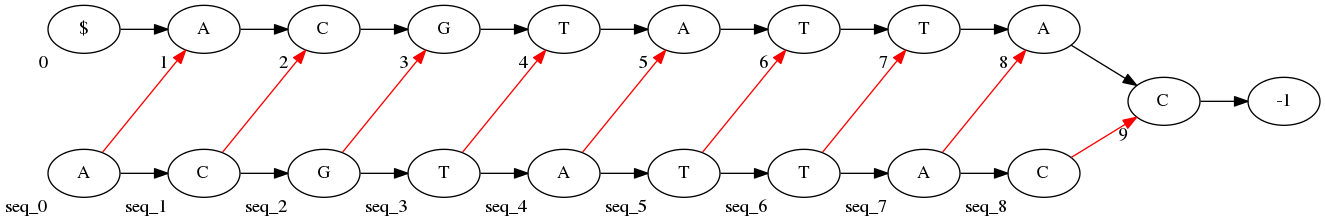
\includegraphics[width=\textwidth]{outputs/equal-alignment.png}
    \end{mdframed}
    \subcaption{}
  \end{subfigure}
  \begin{subfigure}[t]{\textwidth}
    \begin{mdframed}
      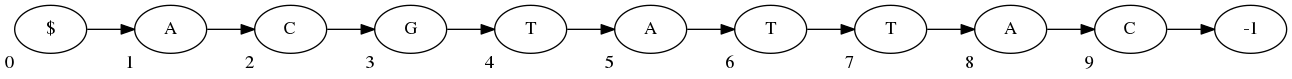
\includegraphics[width=\textwidth]{outputs/equal-merge.png}
    \end{mdframed}
    \subcaption{}
  \end{subfigure}
  \caption{The result of aligning (a) and merging (b) the sequence ``ACGTATTAC'' against the reference graph seen in Fig. \ref{fig:output_ref}}
  \label{fig:output_equal}
\end{figure}
\subsection{SNPs}
\begin{figure}[H]
  \begin{subfigure}[t]{\textwidth}
    \begin{mdframed}
      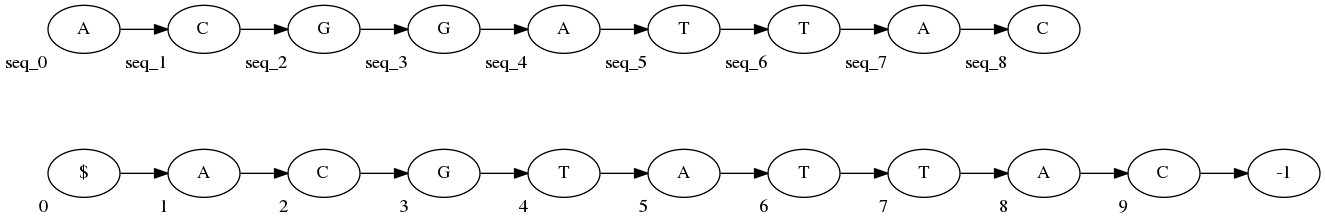
\includegraphics[width=\textwidth]{outputs/snp-no-margin-alignment.png}
    \end{mdframed}
    \subcaption{}
  \end{subfigure}
  \begin{subfigure}[t]{\textwidth}
    \begin{mdframed}
      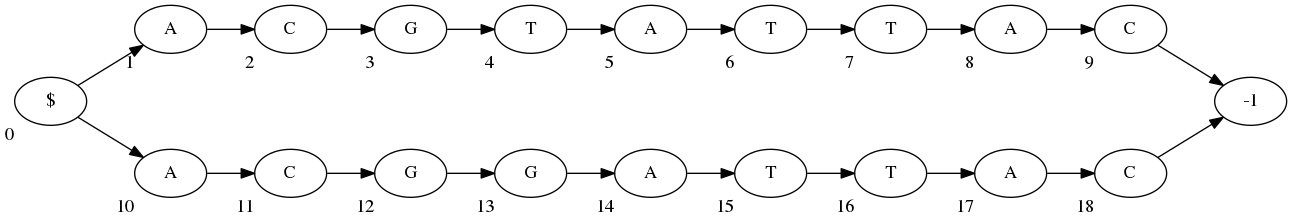
\includegraphics[width=\textwidth]{outputs/snp-no-margin-merge.png}
    \end{mdframed}
    \subcaption{}
  \end{subfigure}
 \caption{The result of aligning (a) and merging (b) the sequence ``ACGGATTAC'' against the reference graph seen in Fig. \ref{fig:output_ref} with $\lambda=0$}
\end{figure}
\begin{figure}[H]
  \begin{subfigure}[t]{\textwidth}
    \begin{mdframed}
      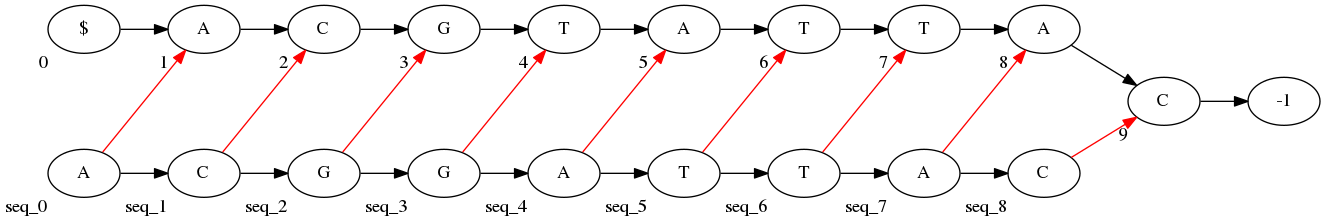
\includegraphics[width=\textwidth]{outputs/snp-alignment.png}
    \end{mdframed}
    \subcaption{}
  \end{subfigure}
  \begin{subfigure}[t]{\textwidth}
    \begin{mdframed}
      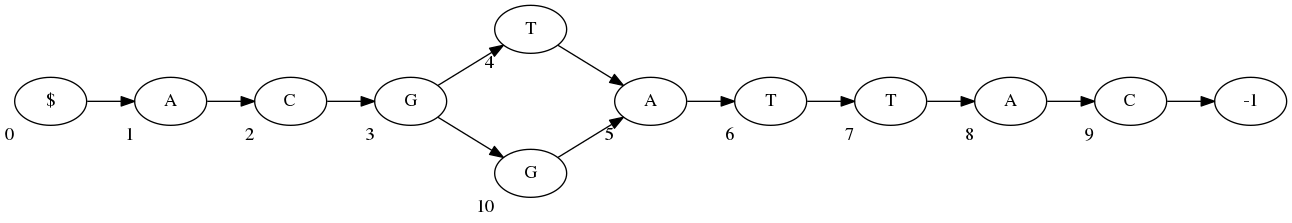
\includegraphics[width=\textwidth]{outputs/snp-merge.png}
    \end{mdframed}
    \subcaption{}
  \end{subfigure}
  \begin{subfigure}[t]{\textwidth}
    \begin{mdframed}
      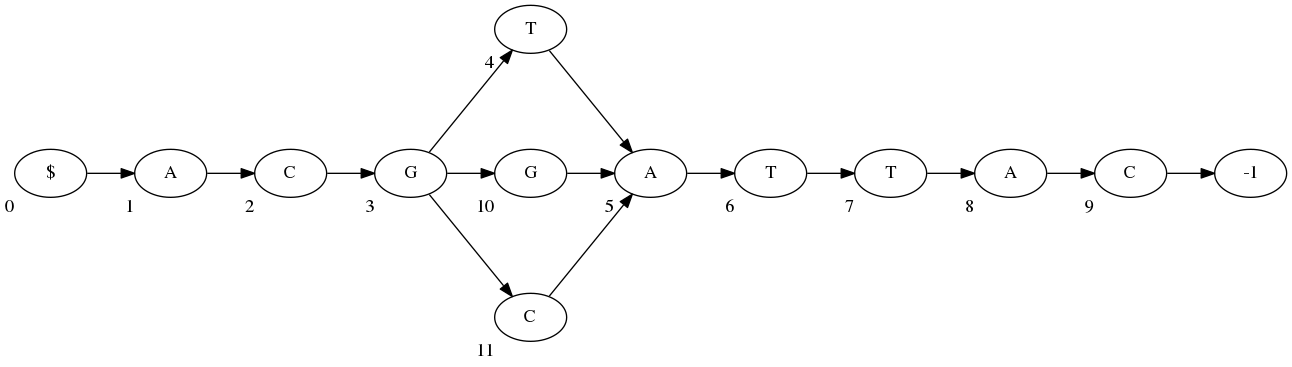
\includegraphics[width=\textwidth]{outputs/snp-merge-two.png}
    \end{mdframed}
    \subcaption{}
  \end{subfigure}
  \caption{The result of aligning (a) and merging (b) the sequence ``ACGGATTAC'' against the reference graph seen in Fig. \ref{fig:output_ref} and then merging the sequence ``ACGCATTAC'' (c) with $\lambda=1$}
  \label{fig:output_snp}
\end{figure}
\subsection{Indels}
\begin{figure}[H]
  \begin{subfigure}[t]{\textwidth}
    \begin{mdframed}
      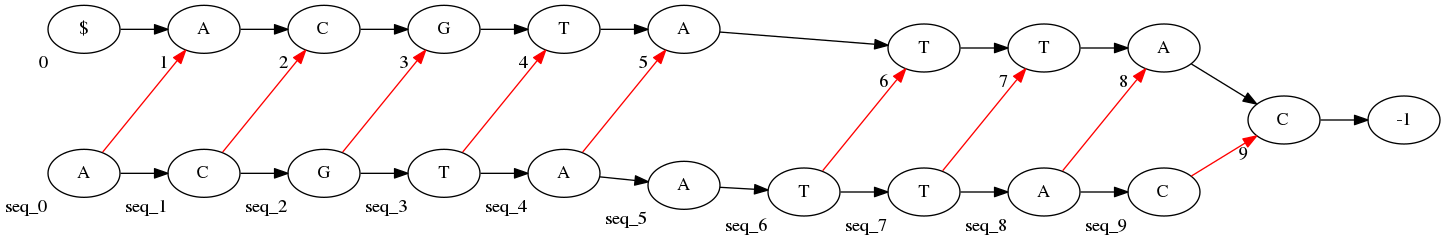
\includegraphics[width=\textwidth]{outputs/insertion-alignment.png}
    \end{mdframed}
    \subcaption{}
  \end{subfigure}
  \begin{subfigure}[t]{\textwidth}
    \begin{mdframed}
      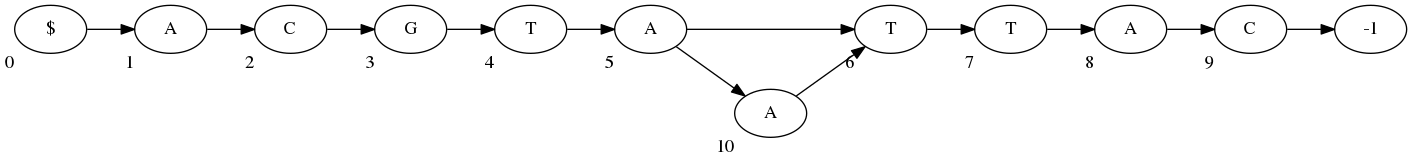
\includegraphics[width=\textwidth]{outputs/insertion-merge.png}
    \end{mdframed}
    \subcaption{}
  \end{subfigure}
  \caption{The result of aligning (a) and merging (b) the sequence ``ACGTAATTAC'' against the reference graph seen in Fig. \ref{fig:output_ref}}
  \label{fig:output_insertion}
\end{figure}
\begin{figure}[H]
  \begin{subfigure}[t]{\textwidth}
    \begin{mdframed}
      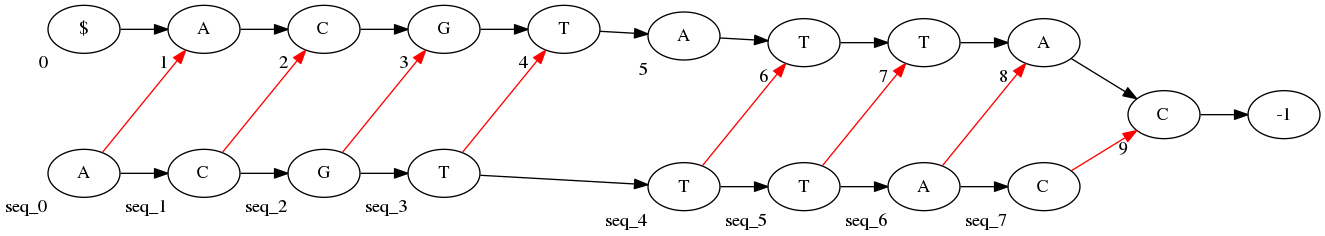
\includegraphics[width=\textwidth]{outputs/deletion-alignment.png}
    \end{mdframed}
    \subcaption{}
  \end{subfigure}
  \begin{subfigure}[t]{\textwidth}
    \begin{mdframed}
      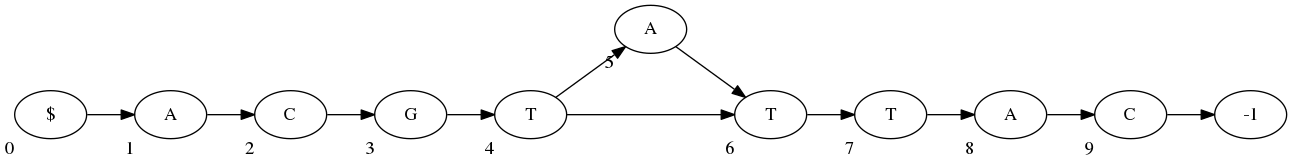
\includegraphics[width=\textwidth]{outputs/deletion-merge.png}
    \end{mdframed}
    \subcaption{}
  \end{subfigure}
  \caption{The result of aligning (a) and merging (b) the sequence ``ACGTTTAC'' against the reference graph seen in Fig. \ref{fig:output_ref}}
  \label{fig:output_deletion}
\end{figure}
\subsection{Structural variation}
\end{document}